\documentclass[tikz,border=12pt]{standalone}
\usepackage[T1]{fontenc}
\usepackage{tgheros}
\renewcommand{\familydefault}{\sfdefault}
\hyphenpenalty=10000
\exhyphenpenalty=10000
\usetikzlibrary{arrows.meta,positioning,calc,backgrounds}
\definecolor{ink}{HTML}{17324D}
\definecolor{muted}{HTML}{526578}
\definecolor{blue}{HTML}{2878A5}
\definecolor{pale}{HTML}{F1F6FA}
\definecolor{safe}{HTML}{237B69}
\definecolor{safefill}{HTML}{EDF7F3}
\definecolor{candidate}{HTML}{A56C16}
\definecolor{candidatefill}{HTML}{FFF7E8}
\definecolor{suspect}{HTML}{AC4D53}
\definecolor{suspectfill}{HTML}{FBF0F0}
\begin{document}
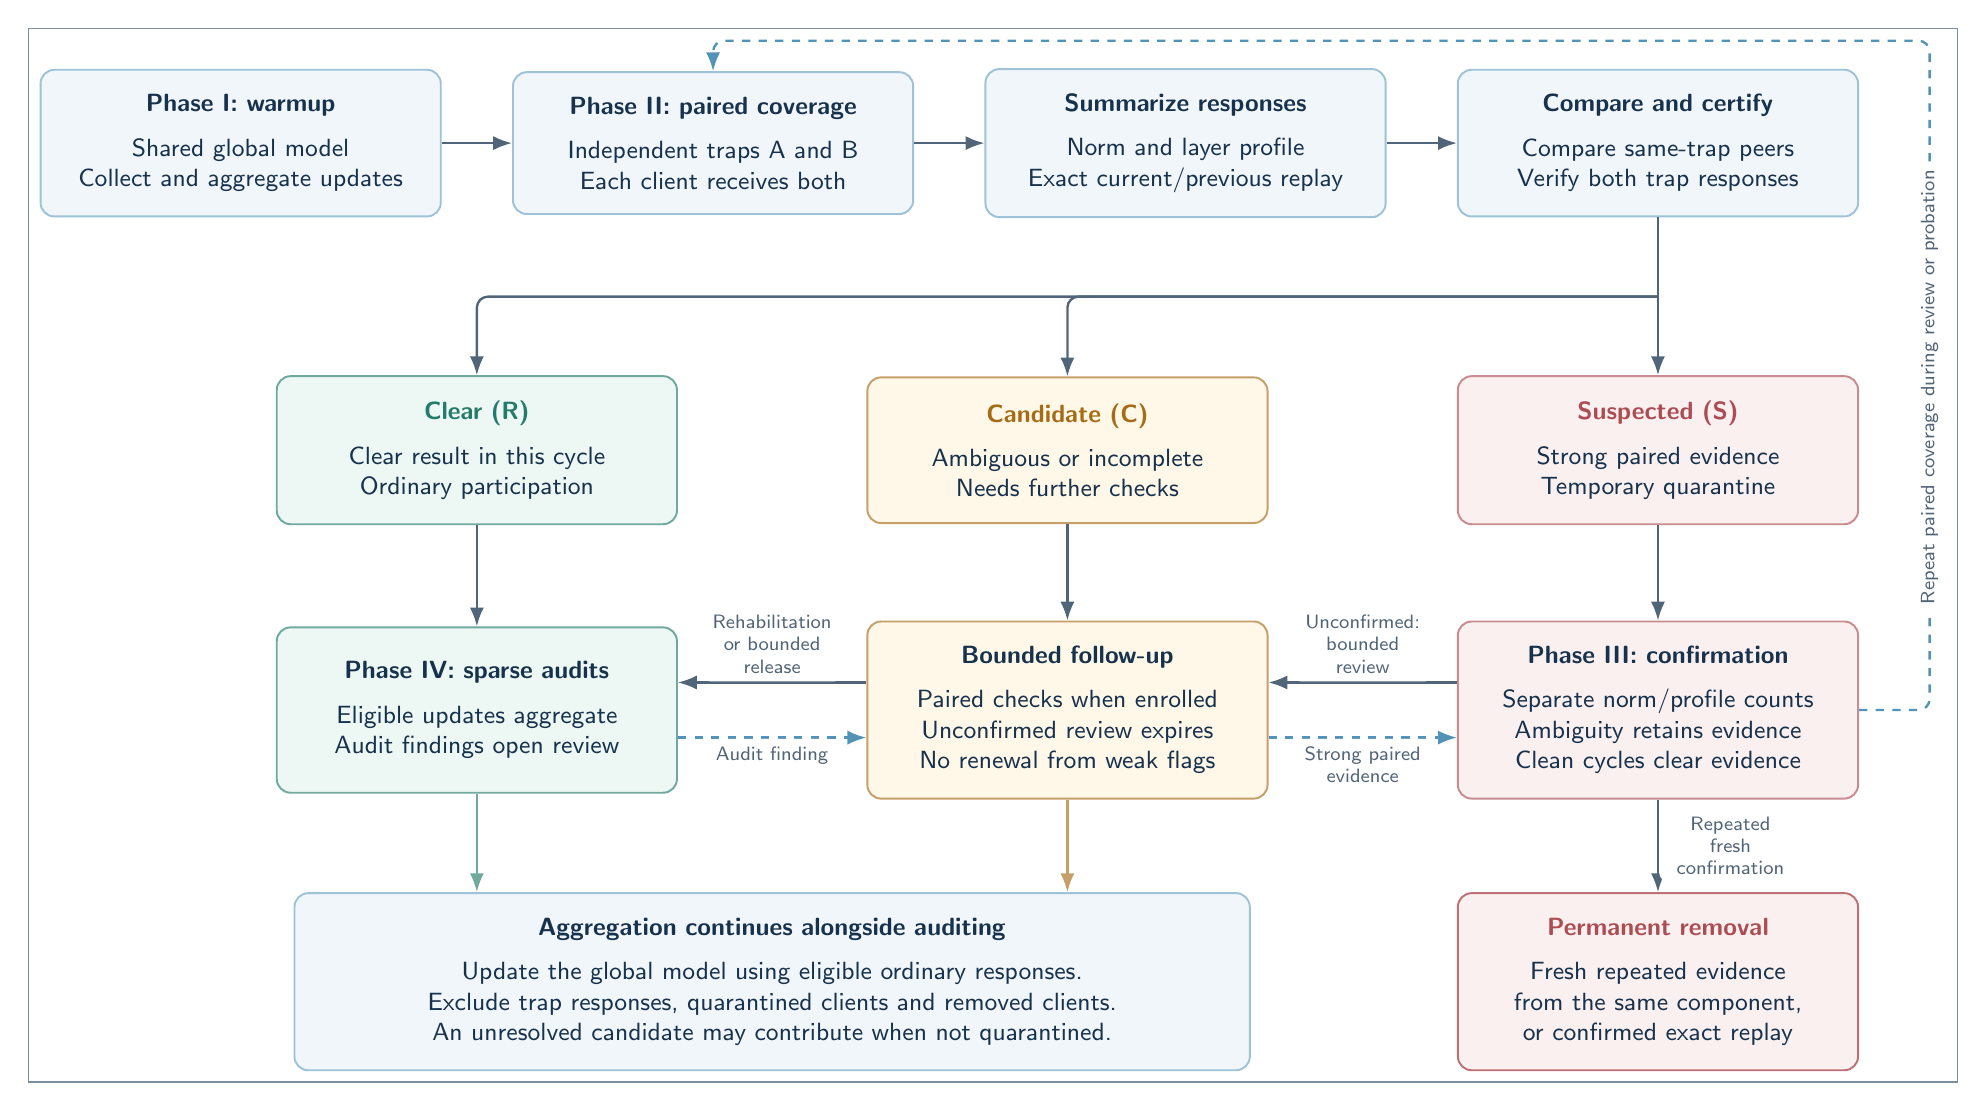
\begin{tikzpicture}[
 font=\sffamily\small,text=ink,
 box/.style={draw=blue!45,fill=pale,rounded corners=5pt,
   line width=.7pt,text width=4.45cm,minimum height=1.75cm,
   align=center,inner sep=9pt},
 state/.style={box,minimum height=1.85cm},
 arrow/.style={-{Latex[length=2.4mm]},draw=ink!75,line width=.85pt,
   rounded corners=4pt},
 feedback/.style={arrow,dashed,draw=blue!80},
 label/.style={font=\sffamily\scriptsize,text=muted,fill=white,inner sep=3pt,align=center}
 ]

\node[box] (warmup) at (0,0)
 {\textbf{Phase I: warmup}\\[5pt]
 Shared global model\\
 Collect and aggregate updates};
\node[box] (traps) at (6,0)
 {\textbf{Phase II: paired coverage}\\[5pt]
 Independent traps A and B\\
 Each client receives both};
\node[box] (measure) at (12,0)
 {\textbf{Summarize responses}\\[5pt]
 Norm and layer profile\\
 Exact current/previous replay};
\node[box] (verify) at (18,0)
 {\textbf{Compare and certify}\\[5pt]
 Compare same-trap peers\\
 Verify both trap responses};
\draw[arrow] (warmup) -- (traps);
\draw[arrow] (traps) -- (measure);
\draw[arrow] (measure) -- (verify);

\node[state,draw=safe!65,fill=safefill] (clear) at (3,-3.9)
 {\textcolor{safe}{\textbf{Clear (R)}}\\[5pt]
 Clear result in this cycle\\
 Ordinary participation};
\node[state,draw=candidate!65,fill=candidatefill] (uncertain) at (10.5,-3.9)
 {\textcolor{candidate}{\textbf{Candidate (C)}}\\[5pt]
 Ambiguous or incomplete\\
 Needs further checks};
\node[state,draw=suspect!65,fill=suspectfill] (strong) at (18,-3.9)
 {\textcolor{suspect}{\textbf{Suspected (S)}}\\[5pt]
 Strong paired evidence\\
 Temporary quarantine};

\coordinate (branch) at (18,-1.95);
\draw[arrow] (verify.south) -- (strong.north);
\draw[arrow] (branch) -| (uncertain.north);
\draw[arrow] (branch) -| (clear.north);

\node[box,draw=safe!65,fill=safefill,minimum height=2.1cm] (routine) at (3,-7.2)
 {\textbf{Phase IV: sparse audits}\\[5pt]
 Eligible updates aggregate\\
 Audit findings open review};
\node[box,draw=candidate!65,fill=candidatefill,minimum height=2.1cm] (review) at (10.5,-7.2)
 {\textbf{Bounded follow-up}\\[5pt]
 Paired checks when enrolled\\
 Unconfirmed review expires\\
 No renewal from weak flags};
\node[box,draw=suspect!65,fill=suspectfill,minimum height=2.1cm] (memory) at (18,-7.2)
 {\textbf{Phase III: confirmation}\\[5pt]
 Separate norm/profile counts\\
 Ambiguity retains evidence\\
 Clean cycles clear evidence};
\draw[arrow] (clear) -- (routine);
\draw[arrow] (uncertain) -- (review);
\draw[arrow] (strong) -- (memory);

\draw[arrow] ([yshift=.35cm]review.west) -- node[label,above,text width=1.65cm]
 {Rehabilitation\\or bounded release} ([yshift=.35cm]routine.east);
\draw[feedback] ([yshift=-.35cm]routine.east) -- node[label,below]
 {Audit finding} ([yshift=-.35cm]review.west);
\draw[arrow] ([yshift=.35cm]memory.west) -- node[label,above,text width=1.65cm]
 {Unconfirmed:\\bounded review} ([yshift=.35cm]review.east);
\draw[feedback] ([yshift=-.35cm]review.east) -- node[label,below,text width=1.65cm]
 {Strong paired\\evidence} ([yshift=-.35cm]memory.west);

\node[box,draw=suspect!80,fill=suspectfill,minimum height=2.05cm] (remove) at (18,-10.65)
 {\textcolor{suspect}{\textbf{Permanent removal}}\\[5pt]
 Fresh repeated evidence\\
 from the same component,\\
 or confirmed exact replay};
\draw[arrow] (memory) -- node[label,right,text width=1.6cm]
 {Repeated fresh\\confirmation} (remove);

% Follow-up and sparse-audit findings lead to new challenges, not a
% repetition of warmup. No single audit can authorize removal.
\coordinate (returntop) at (6,1.3);
\draw[feedback] (memory.east) -- (21.45,-7.2) -- (21.45,1.3)
 -- (returntop) -- (traps.north);
\node[label,rotate=90] at (21.45,-3.1) {Repeat paired coverage during review or probation};

\node[box,draw=blue!45,fill=pale,text width=11.5cm,
 minimum height=2.05cm] (aggregation) at (6.75,-10.65)
 {\textbf{Aggregation continues alongside auditing}\\[5pt]
 Update the global model using eligible ordinary responses.\\
 Exclude trap responses, quarantined clients and removed clients.\\
 An unresolved candidate may contribute when not quarantined.};
\draw[arrow,draw=safe!65] (routine.south) -- (3,-9.05) -- (aggregation.north -| 3,0);
\draw[arrow,draw=candidate!65] (review.south) -- (10.5,-9.05) -- (aggregation.north -| 10.5,0);

\begin{scope}[on background layer]
 \draw[ink!55,line width=.6pt]
  ([xshift=-4pt,yshift=-4pt]current bounding box.south west)
  rectangle ([xshift=4pt,yshift=4pt]current bounding box.north east);
\end{scope}
\end{tikzpicture}
\end{document}
